\subsection{Pruebas de la versión: 4} \label{chp:pruebasV1}
En esta sección se describen los resultadods de las pruebas realizadas de la cuarta versión del algoritmo de optimización de horarios.\\

Como consideración tenemos que las pruebas fueron realizadas en una laptop dell Inspiron 15 con procesador intel i5 5ta generación 4gb de memoria ram usando el sistema operativo debian 9.\\


\subsubsection{Pruebas realizadas}

Inicialmente las funciones que comprenden el algoritmo fueron modificadas de su funcionamiento en los prototipos anteriores para funcionar con la base de datos y la población completa por lo que se corroboró el funcionamiento de dichas funciones. \\

\begin{itemize}
	\item Se corroboró que la función de generar Población utilizara todas las opciones de Materia-Profesor disponibles y que el resultado tuviera la estructura que hemos definido. 
	
	\item Se probó la función de evaluación, para corroborar que las restricciones ingresadas sean tomadas en cuenta al momento de asignar una calificación a un horario.
	
	\item Se probó la función de crear la población evaluada de manera que se cree el número de individuos(horarios) que se requieren.
	
	\item Se probaron las funciones de mutación de forma que el resultado arrojado después de llevar a cabo dichos operadores sea en realidad distinto a la entrada del mismo así como se corroboró que se llevaran a cabo de la manera esperada.
	
\end{itemize}

Una vez que se corrigieron los errores arrojados por las pruebas de cada función por separado, las funciones fueron integradas para ser utilizadas en conjunto. Para corroborar que el funcionamiento fuera correcto, utilizamos la estructura educativa actual de la ESCOM para el semestre 2019/1. Utilizando estos datos, se crearon 15 individuos dentro de la población inicial y se les dio una evaluación.\\

Una vez que se operaron las funciones de mutación sobre la población generada por nuestra función de generar Población, se logró disminuir la calificación del primer individuo por debajo de la calificación de la estructura actual de ESCOM alrededor de las 1500 iteraciones por lo cual esto fue considerado un criterio de paro.\\


Se tomó la calificación de los mejores 5 individuos de la población inicial por cada 100 iteraciones para comprobar la mejora. En la figura \ref{fig:PruebaV4} se muestran los resultados del experimento y en la figura \ref{fig:grafV4} se muestra la gráfica de los mismos donde se puede apreciar que a partir de las 1,500 iteraciones los individuos de la población alcanzan mejores calificaciones que la calificación de la estructura educativa actual.\\
 
 \begin{figure}[htbp!]
 	\begin{center}
 		\fbox{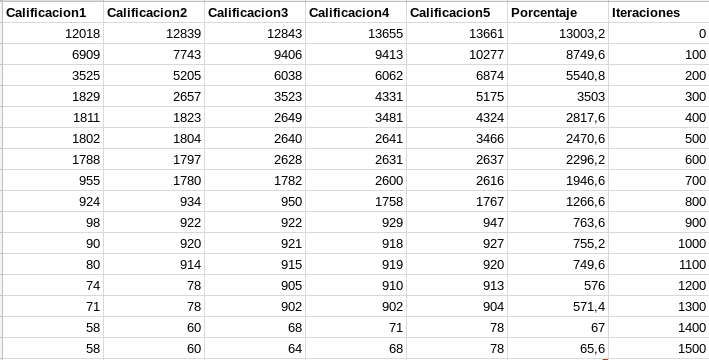
\includegraphics[width=.7\textwidth]{ModeloComportamiento/Algoritmo/imagenes/tabla4.png}}
 		\caption{Determinación experimental del criterio de paro}
 		\label{fig:PruebaV4}
 	\end{center}
 \end{figure}


\begin{figure}[htbp!]
	\begin{center}
	\fbox{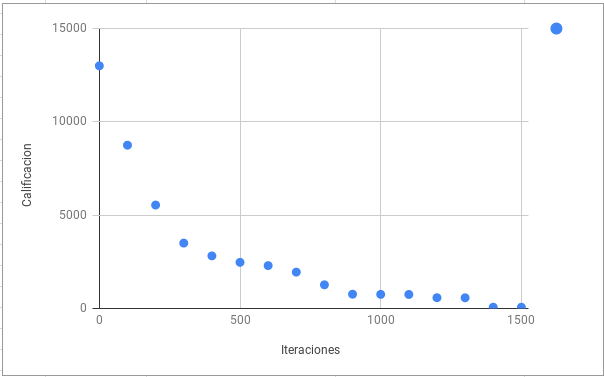
\includegraphics[width=.7\textwidth]{ModeloComportamiento/Algoritmo/imagenes/grafica4.png}}
		\caption{Gráfica de mejora}
		\label{fig:grafV4}
	\end{center}
\end{figure}

